\chapter{Virtual Try-on}
\label{chapter-virtual-tryon}
\begin{ChapAbstract}
In this chapter, we propose Distilled Mobile Real-time Virtual Try-On (DM-VTON), which focuses on synthesizing try-on images with increased speed compared to previous methods while ensuring accuracy. Our approach is based on a knowledge distillation scheme that leverages a strong Teacher network as supervision to guide a Student network without relying on human parsing. Notably, we introduce an efficient Mobile Generative Module within the Student network, significantly reducing the runtime while ensuring high-quality output. Additionally, we propose Virtual Try-on-guided Pose for Data Synthesis to address the limited pose variation observed in training images. Finally, we provide the experimental details of our proposed method, and then we present a comparative study of DM-VTON with state-of-the-art methods.
\end{ChapAbstract}

%%%%%%%%%%%%%%%%%%%%%%%%%%%%%%%%%%%%%%%%%%%%%%%%%%%%%%%%%%%%%%%%
\section{Overview}
\begin{figure}[h!]
  \centering
  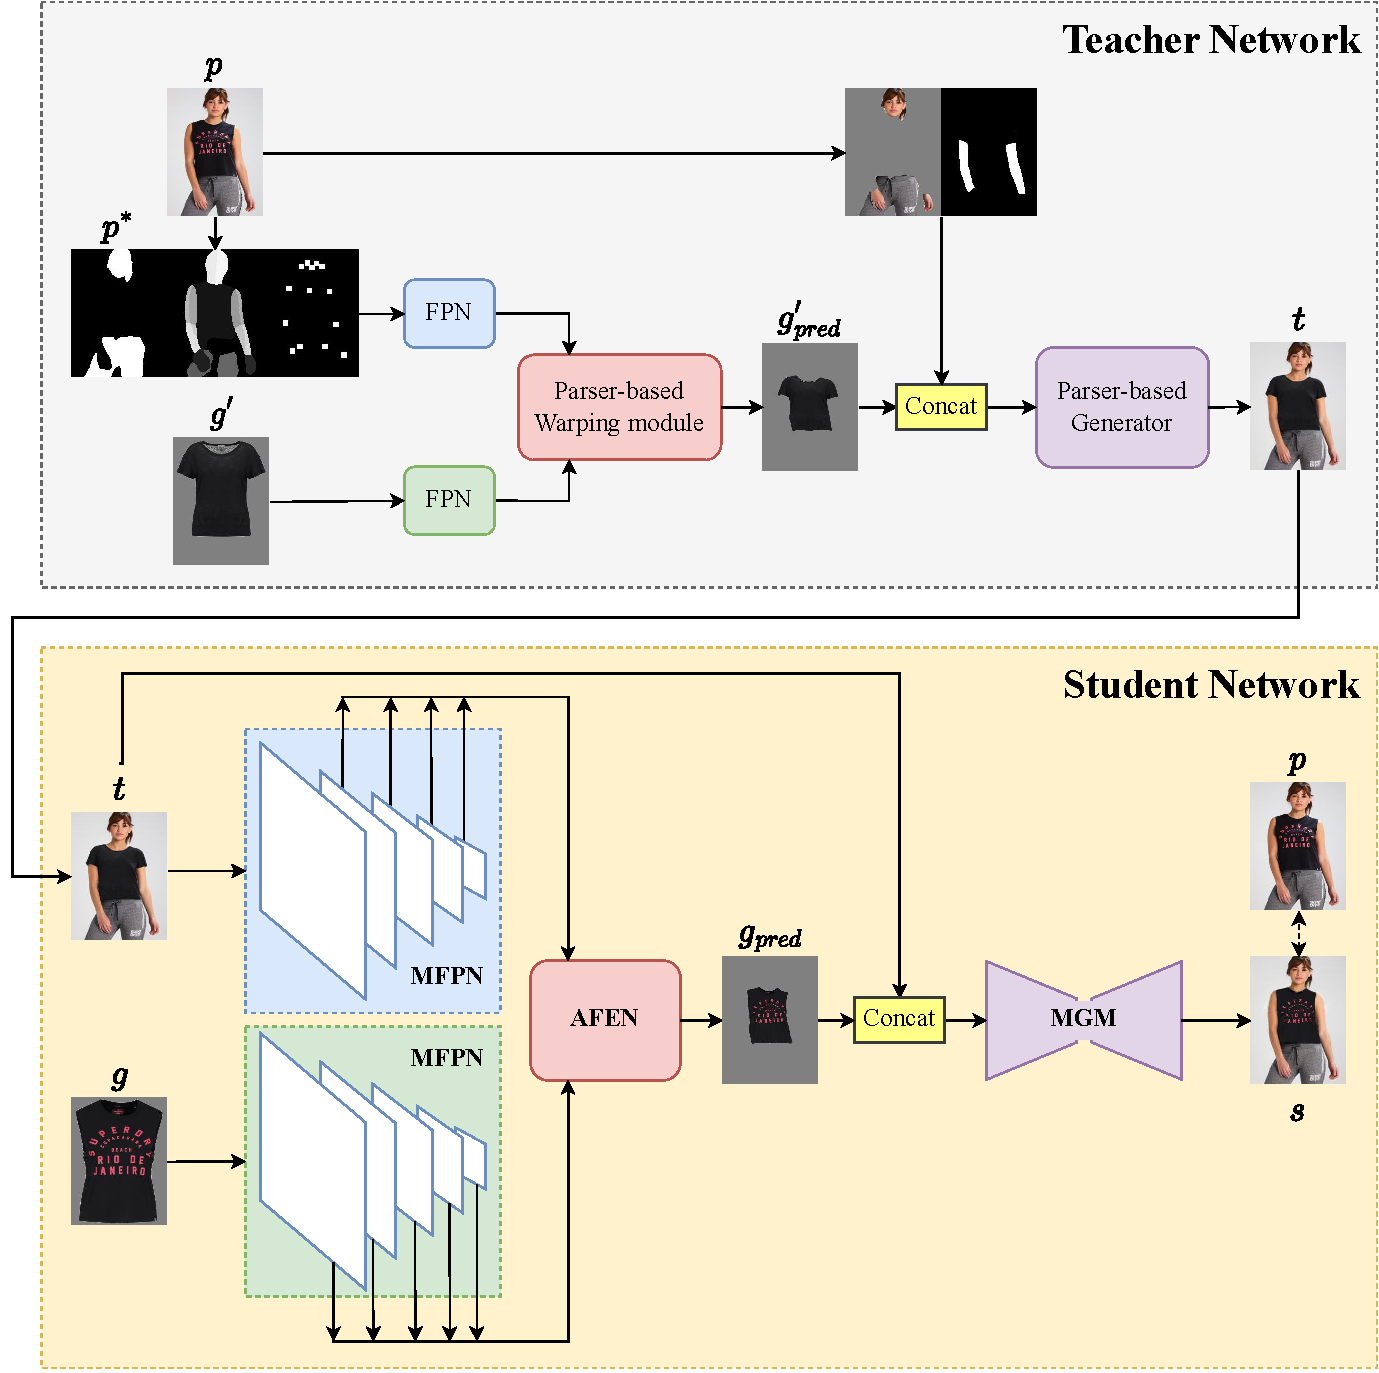
\includegraphics[width=\textwidth]{content/resources/images/tryon/mobile-tryon.pdf}
  \caption{Overview architecture of the proposed Distilled Mobile Real-time Virtual Try-On (DM-VTON) framework. The parser-based Teacher network generates a synthetic image as the input for training the Student network.}
  \label{fig:mobile-tryon}
  \vspace{-1mm}
\end{figure}

Our objective is to generate an image of a person wearing a specific garment while preserving the rest of the image. To achieve this goal, we adopt the knowledge distillation training pipeline~\cite{Hinton-Arxiv2015-Distilling, Issenhuth-ECCV2020-Do, Ge-CVPR2021-Parser, He-CVPR2022-Style, Lin-IJCAI2022-RMGN} to develop a Distilled Mobile Real-time Virtual Try-On (DM-VTON) framework (see~\autoref{fig:mobile-tryon}). Our proposed DM-VTON consists of two networks: Teacher and Student networks. Both include several main components: feature extractor, clothes-warping module, and generator. 


The Teacher network aims to produce the virtual try-on result using the parser-based training process. The Student network then utilizes the Teacher network to generate synthetic input images, enabling the Student network to be supervised by the original images without relying on human representation. The Teacher network is built upon SOTA virtual try-on models to ensure high-quality output. Focusing on inference speed, we propose lightweight components for the Student network. 

%%%%%%%%%%%%%%%%%%%%%%%%%%%%%% 
\section{Appearance Flow}
The concept of appearance flow begins with a method for synthesizing images of the same object observed from arbitrary viewpoints introduced by Zhou et al.~\cite{Zhou-ECCV2016-AppearanceFlow}. From the observation that the appearance (texture, shape, colour, etc.) of different views of an object are highly correlated, research suggests that the information of an input view can be used to generate images for various views. Appearance flow refers to 2-D coordinate vectors specifying which pixels in the input view could be used to synthesize the target view. Specifically, with the pixel $i$ of the target image, the appearance flow vector $f^i \in \mathbb{R}^2$ indicates the coordinate of the input pixel sampled to reconstruct it (as illustrated in~\autoref{fig:appearance-flow-ex}). This idea is also applied to solve many problems, such as visual tracking~\cite{Song-ICCV2017-Crest}, pose transfer~\cite{Li-CVPR2019-Dense}, image inpainting~\cite{Liu-ECCV2020-Rethinking}, virtual try-on~\cite{Ge-CVPR2021-Parser, He-CVPR2022-Style}

\begin{figure}[h]
    \centering
    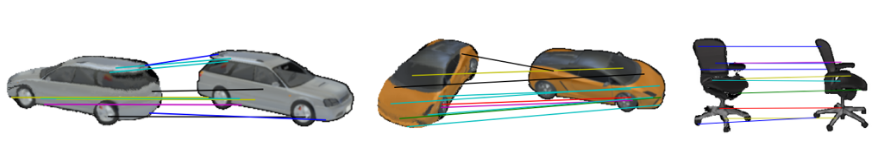
\includegraphics[width=\linewidth]{content/resources/images/tryon/appearance-flow-ex.png}
    \caption{Illustration of appearance flow vectors (Source: View Synthesis by Appearance Flow~\cite{Zhou-ECCV2016-AppearanceFlow}).}
    \label{fig:appearance-flow-ex}
\end{figure}

%%%%%%%%%%%%%%%%%%%%%%%%%%%%%% 
\section{Teacher Network}

The main purpose of this network is to generate a synthetic person image that serves as the input for the Student training process. Furthermore, the Teacher also helps this process through a knowledge distillation scheme. In particular, we take advantage of the SOTA method of virtual try-on task: FS-VTON \cite{He-CVPR2022-Style}. As shown in~\autoref{fig:mobile-tryon}, it incorporates two feature pyramid networks (FPN)~\cite{Lin-CVPR2017-FPN} constructed from residual blocks, enabling the extraction of features from the human representation $p^*$ and garment image $g'$. To achieve the garment deformation functionality, the Teacher network utilizes a style-based global appearance flow estimation network that uses modulated convolution \cite{Karras-CVPR2019-Style}. This network first predicts a coarse appearance flow via extracted global style vector and then refines it locally. The last flow thus can capture the global and local correspondence between the garment and the target person. This makes the Teacher network more robust against the problems of detail-preserving and large misalignment. Finally, the warped clothes and the preserved region on the human body are concatenated as the generator input for try-on result generation. The generator of our Teacher network follows the encoder-decoder architecture with skip connections, which have been proven effective in detail preservation.

Because the inputs of the parser-based model (i.e., human representation) contain more semantic information when compared to those in the parser-free model, we employ an adjustable knowledge distillation learning scheme~\cite{Ge-CVPR2021-Parser} with a distillation loss to guide the Student network. When training the Student network with fake image $t$ and garment $g$, we also pass $p*$ and $g$ through the pretrained Teacher network. The distillation loss is formulated as follows:
\begin{align}
    L_{dis}  & = \lambda_{fea}L_{fea} + \lambda_{flow}L_{flow},\\
    L_{fea}  & = \psi \sum_{i=1}^N(p^{pb}_{i} - t^{pf}_{i})^2 + \psi \sum_{i=1}^N(g^{pb}_{i} - g^{pf}_{i})^2,\\
    L_{flow} & = \psi \sum_{i=1}^N\|f^{pb}_{i} - f^{pf}_{i}\|_{2},\\
    \psi     & = \{\begin{array}{l} 1, ~if~ \|t-p\|_1<\|s-p\|_1 \\ 0,~otherwise \end{array},
\end{align}
where $t$, and $s$ are the try-on result of the Teacher and Student, respectively; $p$ is the person image ground truth. $p^{pb}_{i}$ and $t^{pf}_{i}$ denote the output feature maps at the $i$-th scale extracted from $p*$ and fake image $t$; similarly, $g^{pb}_{i}$ and $g^{pf}_{i}$ are the $i$-th scale feature maps extracted from garment image $g$ by the feature extractor of parser-based and parser-free network, respectively. $f^{pb}_{i}$ and $f^{pf}_{i}$ are the predicted appearance flows from the Teacher and Student warping modules at the $i$-th scale. $\psi$ is the adjustable factor used to adjust so that the distilling process takes place only if the quality of the generated image of the parser-based network is better than that of the parser-free network.

%%%%%%%%%%%%%%%%%%%%%%%%%%%%%% 
\section{Student Network}

We propose a parser-based approach for synthesizing try-on images with increased speed compared to previous methods while ensuring accuracy. As shown in~\autoref{fig:mobile-tryon}, our Student network consists of three key components: Mobile Feature Pyramid Network (MFPN), Appearance Flow Estimation Network (AFEN), and Mobile Generative Module (MGM). These components synergistically collaborate to extract features, manipulate garments through deformation, and generate try-on images. The AFEN introduced by Ge et al.~\cite{Ge-CVPR2021-Parser} proved effective in deforming garments by using appearance flow estimates from pyramid features. The MFPN and MGM are built upon the architecture of MobileNetV2~\cite{Sandler-CVPR2018-Mobilenetv2} with Inverted Residual blocks specifically designed to optimize computational efficiency and model size.

%%%%%%%%%%%%%%%%%%%%%%%%%%%%%% 
\subsection{Mobile Feature Pyramid Network}
% \footnote{https://github.com/libiseller/MobileNetV2-dynamicFPN}
As shown in~\autoref{fig:mobile-pyramid}, MFPN incorporates the architecture of MobileNetV2 with Inverted Residual blocks~\cite{Sandler-CVPR2018-Mobilenetv2} to a Feature Pyramid Network. By leveraging the capabilities of two MFPN blocks, we extract two-branch N-level feature maps from person and garment images within a parser-free network. These features are fed into the Appearance Flow Estimation Network (AFEN) to predict the appearance flow map for garment deformation.

\begin{figure}[h!]
  \centering
  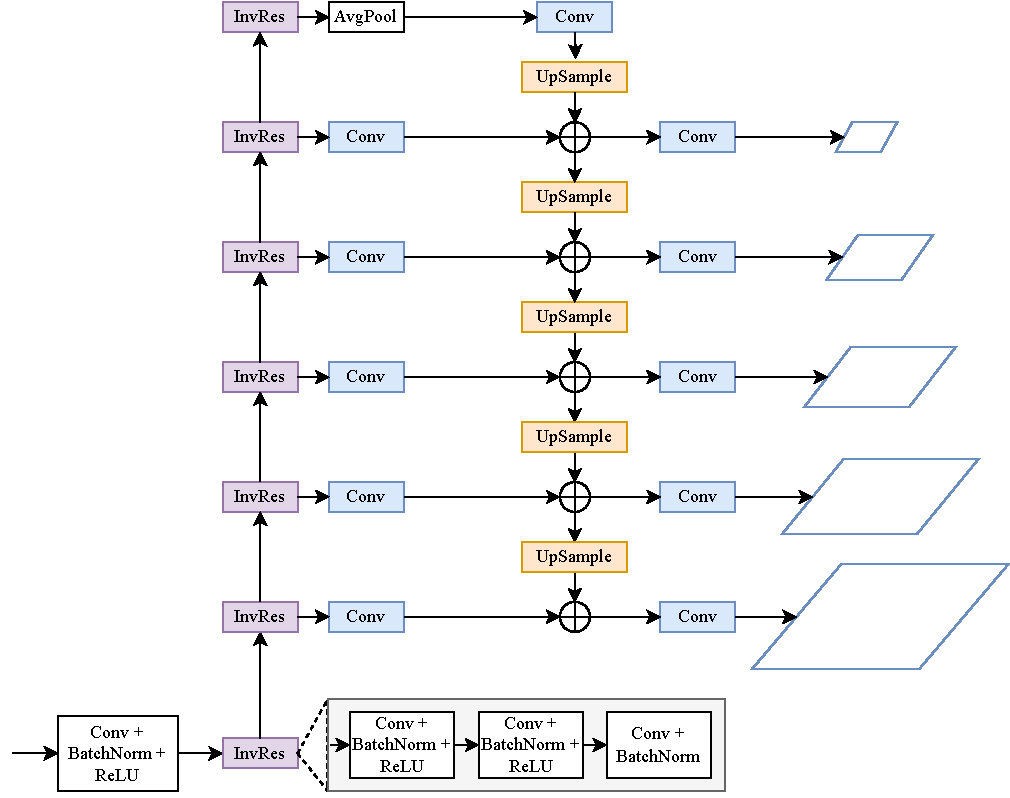
\includegraphics[width=\linewidth]{content/resources/images/tryon/mobile-pyramid.pdf}
  \caption{Mobile Feature Pyramid Network architecture}
  \label{fig:mobile-pyramid}
  \vspace{-2mm}
\end{figure}

%%%%%%%%%%%%%%%%%%%%%%%%%%%%%% 
\subsection{Appearance Flow Estimation Network}
This component aims to deform the garment to fit the human pose while preserving the texture. Following the work of Ge et al.~\cite{Ge-CVPR2021-Parser}, we adopt an appearance flow estimation network (AFEN) comprising subnetworks equipped with varying sizes of convolution layers. These subnetworks are responsible for estimating flows based on extracted multi-level feature maps. The outcome of this network can capture the long-range correspondence between the garment image and the person image, effectively minimizing issues related to misalignment. To enhance the preservation of clothing characteristics, this module is optimized with the second-order constraint:
\begin{equation} 
L_{sec}=\sum_{i=1}^N \sum_t \sum_{\pi \in N_t} CharLoss\left(f_i^{t-\pi}+f_i^{t+\pi}-2 f_i^t\right),
\end{equation}
where $f_i^t$ denotes the $t$-th point on the $i$-th scale flow map; $N_t$ is the set of horizontal, vertical, and diagonal neighborhoods around the $t$-th point; and $CharLoss$ denotes generalized Charbonnier loss~\cite{Sun-IJCV2014-Quantitative}.

%%%%%%%%%%%%%%%%%%%%%%%%%%%%%% 
\subsection{Mobile Generative Module}
To synthesize the entire try-on image from the warped image and target person image, we develop a Mobile Generative Module, the integration of the architectural principles of UNet~\cite{Ronneberger-MICCAI2015-Unet} and MobileNetV2~\cite{Sandler-CVPR2018-Mobilenetv2} as illustrated in~\autoref{fig:mobile-unet}. The primary objective behind the design of this generator is to reduce both the computational burden and the model's overall size.

\begin{figure}[h!]
  \centering
  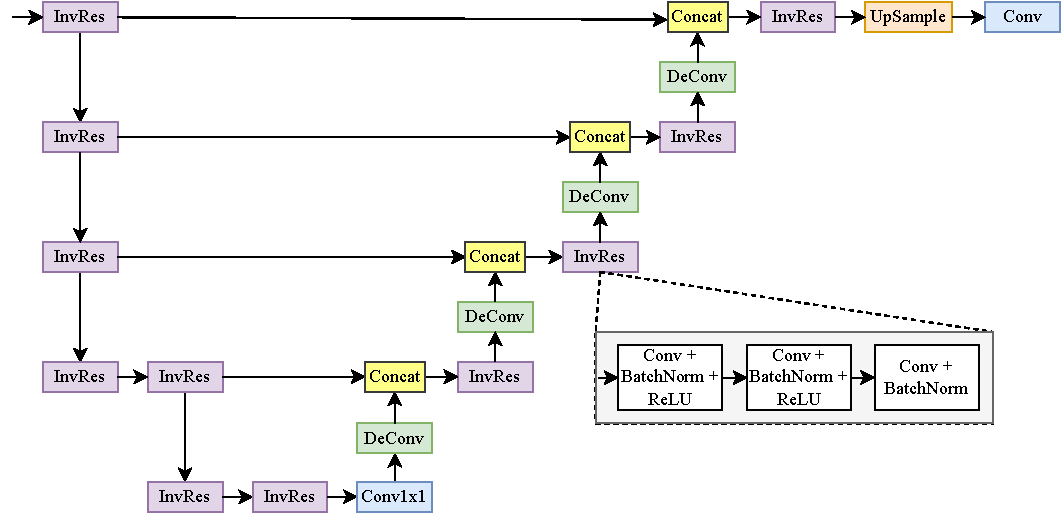
\includegraphics[width=\linewidth]{content/resources/images/tryon/mobile-unet.pdf}
  \caption{Mobile Generative Module architecture}
  \label{fig:mobile-unet}
  \vspace{-2mm}
\end{figure}

%%%%%%%%%%%%%%%%%%%%%%%%%%%%%% 
\subsection{Loss Function}
During training, we optimize the warping module separately in the first stage and then train together with the generator in the last stage. The loss function used in the first stage is defined as:
\begin{align}
    L^{warp} & = \lambda^{warp}_{l}L^{warp}_{l} + \lambda^{warp}_{per}L^{warp}_{per} + \lambda_{sec}L_{sec} + \lambda_{dis}L_{dis},\\
    L^{warp}_{l} & = \|g_{pred} - p \odot m_{gt}\|,\\
    L^{warp}_{per} & = \sum_i{\|\Phi_i(g_{pred}) - \Phi_i(p \odot m_{gt})\|},
\end{align}
where $L^{warp}_{l}$ denotes pixel-wise L1 loss, $L^{warp}_{per}$ is the perceptual loss~\cite{Johnson-ECCV2016-Perceptual}, $L^{warp}_{sec}$ is the smooth loss (second-order constrain), $L^{warp}_{dis}$ is the distillation loss, $g_{pred}$ is warped garment.  $p$ is the person image ground truth with the garment mask $m_{gt}$; $\Phi_i$ denotes the $i$-th block of pre-trained VGG19~\cite{Simonyan-ArXiv2014-VGG}.

With the generative module, we also apply L1 loss perceptual loss~\cite{Johnson-ECCV2016-Perceptual} between the synthesized image and the ground truth image to supervise the training process of MGM:
\begin{align}
    L^{gen} & = \lambda^{gen}_{l}L^{gen}_{l} + \lambda^{gen}_{per}L^{gen}_{per},\\
    L^{gen}_{l} & = \|s - p\|,\\
    L^{gen}_{per} & = \sum_i{\|\Phi_i(s) - \Phi_i(p)\|},
\end{align}
where $L^{gen}_{l}$ is L1 loss and $L^{gen}_{per}$ is the perceptual loss~\cite{Johnson-ECCV2016-Perceptual}. $s$ and $p$ are the generated output of the Student network and the person image ground truth, respectively. 

In practice, we empirically set $\lambda^{warp}_{l}$ = 1, $\lambda^{warp}_{per}$ = 0.2, $L^{warp}_{sec}$ = 6, $L^{warp}_{dis}$ = 0.04, $\lambda^{gen}_{l}$ = 5,
 $\lambda^{gen}_{per}$ = 1. The overall loss function 
when training the whole model in the last stage is:
\begin{align}
    L & = 0.25*L^{warp} + L^{gen}.
\end{align}

\section{Virtual Try-on-guided Pose for Data Synthesis}

By using the K-Means clustering algorithm, we observe that the original VITON dataset~\cite{Han-CVPR2018-Viton} is mainly composed of images with straight-arm poses (as in~\autoref{fig:pose-distribution}(a)). This bias creates a challenge as models trained on such data are prone to overfit and perform poorly on images with different upper-body poses. To tackle this problem, we propose the Virtual Try-on-guided Pose for Data Synthesis (VTP-DS) pipeline. Intending to improve the existing virtual try-on framework, the pipeline incorporates two key ideas: automatically detecting poorly performed poses using the Object Keypoint Similarity (OKS) metric~\cite{Lin-ECCV2014-Microsoft} and synthesizing new training data specifically targeting those poses. The overview of the VTP-DS pipeline is illustrated in~\autoref{fig:augment-pipeline}.

\begin{figure}[h!]
 \centering 
 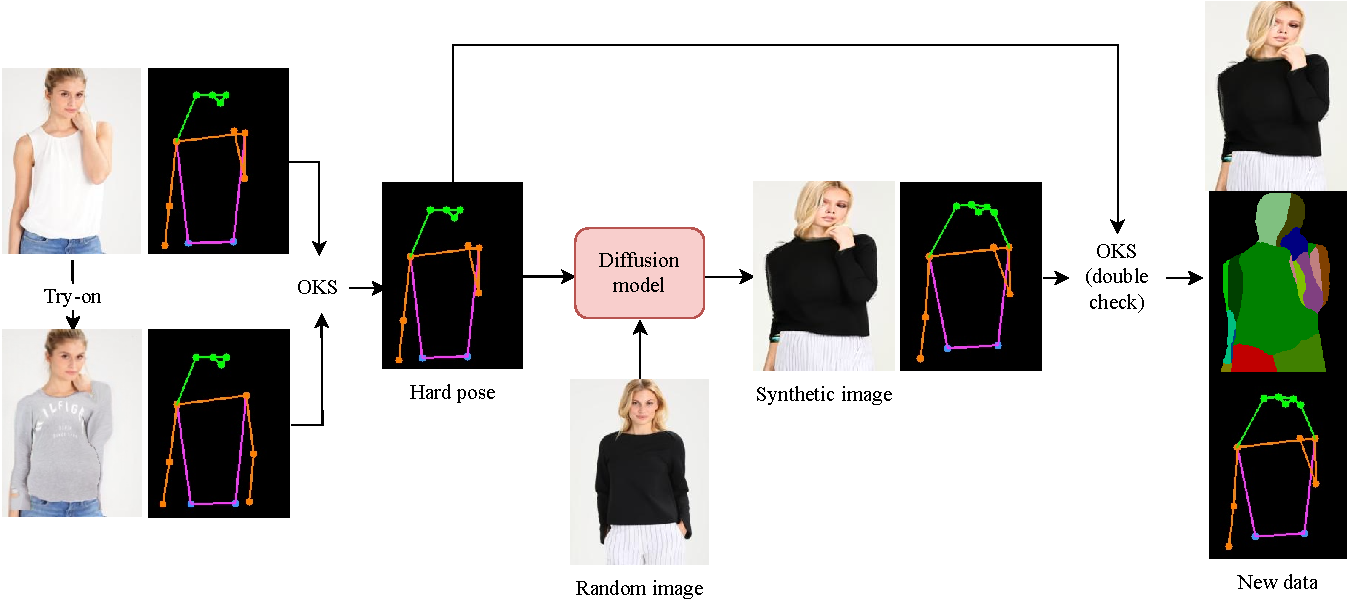
\includegraphics[scale=0.55]{content/resources/images/tryon/augment-pipeline.pdf}
  \caption{Overview of Virtual Try-on-guided Pose for Data Synthesis pipeline.}
   \label{fig:augment-pipeline}
   \vspace{-2mm}
\end{figure}

\begin{figure}[h!]
    \centering
    \subfloat[VITON]{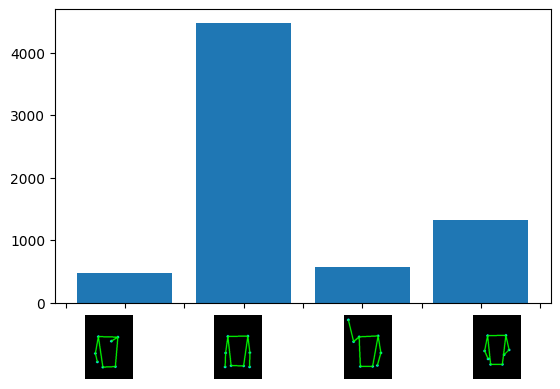
\includegraphics[width=0.45\columnwidth]{content/resources/images/tryon/viton-clean.png}}
    \subfloat[VITON + synthesized data]{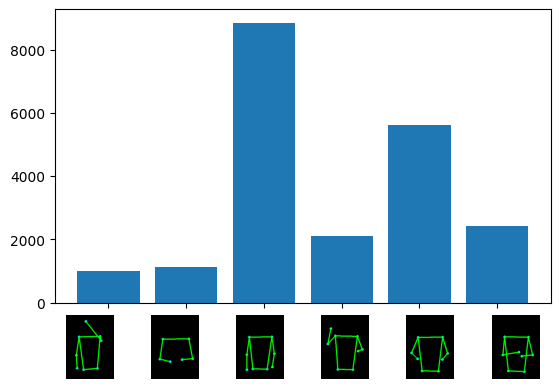
\includegraphics[width=0.45\columnwidth]{content/resources/images/tryon/merge1.png}} 
    \caption{Pose distribution in VITON dataset~\cite{Han-CVPR2018-Viton}.}
    \label{fig:pose-distribution}
    \vspace{-2mm}
\end{figure}

Given an input image containing a person, we extract that person's pose by using the YOLOv7 pose estimation method~\cite{Wang-CVPR2023-YOLOv7}. Then, we utilize our trained DM-VTON model to perform virtual try-on on the input image. The extracted pose from the resulting image is compared with the pose of the input image using a customized OKS metric ~\autoref{formulat:oks}.  

\begin{equation}
    \centering
    \frac{1}{|P|}\sum_{i \in P} \exp(\frac{-d_i^2}{2 s^2 k_i^2}),
    \label{formulat:oks}
\end{equation}
where $P$ denotes the set of arm and hand keypoints, while the original formula uses all keypoints; $d_i$ denotes the Euclidean distance between the keypoint $i$ of two poses; $s$ denotes the total area containing the pose; $k_i$ is the constant provided by Lin et al.~\cite{Lin-ECCV2014-Microsoft} to represent the standard deviation for keypoint $i$. Because we focus on distinguishing different upper-body poses, only the arm and hand keypoints contribute to the formula. If the OKS score falls below a specified threshold $t=0.9$, it is identified as a hard pose.

Once identifying a hard pose, we randomly pick a person image from the VITON dataset. Then it leverages Bhunia's Diffusion model~\cite{Bhunia-CVPR2023-Person} to synthesize a new image of the person in the corresponding pose. To ensure the accuracy of the synthesized image, we perform a double-check using the OKS metric to verify the correctness of the output pose. Finally, DensePose~\cite{Guler-CVPR2018-DensePose} is utilized to generate the body-parser map of the synthesized image.

We initially collected videos from Youtube to synthesize additional data for training networks, specifically focusing on posing or catwalk videos. These videos had varying durations, ranging from 1 to 10 minutes. Subsequently, we extracted individual frames from these videos, which served as the input for our VTP-DS pipeline. %The threshold $t$ for the Object Keypoints Similarity (OKS) metric is set to 0.9. 
After that, we manually removed low-quality results, resulting in 14,314 high-quality synthesized images for training the networks. 

To access the quality of synthesized images, we use the K-means algorithm combined with our modified OKS metric. As details of the pose clustering results shown in~\autoref{fig:pose-distribution}, data in the VITON training set mainly focuses on poses with simple poses (i.e. arms are less covered, low rotation amplitude). Meanwhile, when combined with our synthesized images, new pose clusters appear, and the concentration of data in groups is less imbalanced, which can help to train robust virtual try-on models. 

%%%%%%%%%%%%%%%%%%%%%%%%%%%%%%%%%%%%%%%%%%%%%%%%%%%%%%%%%%%%%%%%
\section{Experiments}
\begin{figure}[h!]
  \centering
  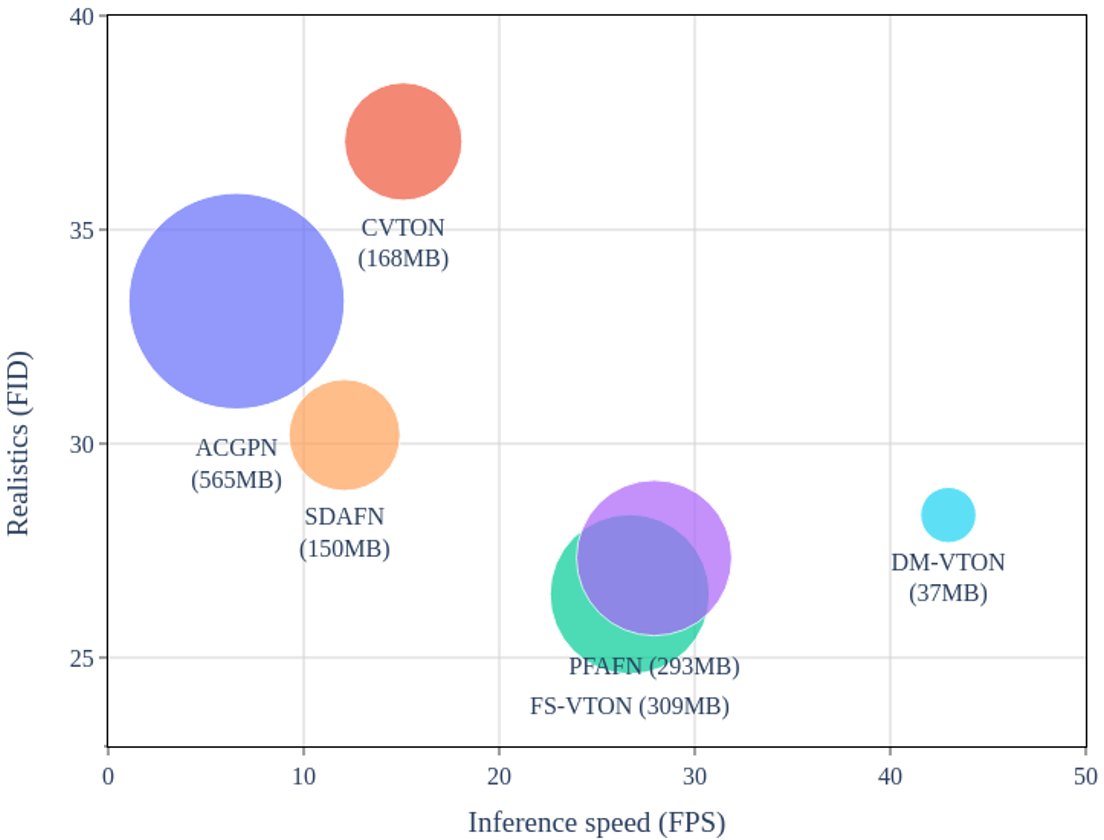
\includegraphics[width=\linewidth]{content/resources/images/tryon/teaser.png}
  \caption{The comparison of our method (DM-VTON) and SOTA methods on VITON test set~\cite{Han-CVPR2018-Viton} in terms of realistic results (FID~\cite{Heusel-NeurIPS2017-FID}, lower is better), inference speed (FPS, higher is better), and memory usage. The size of each bubble represents the memory footprint. FPS is measured using a single Nvidia Tesla T4 GPU.}
  \label{fig:teaser}
  \vspace{-1mm}
\end{figure}

We conducted experiments comparing our DM-VTON framework with other state-of-the-art (SOTA) methods in terms of inference speed, memory usage, and the realisticness of the output. During the experimentation, we carefully evaluated the trade-off between those factors. As depicted in~\autoref{fig:teaser}, our DM-VTON framework outperforms all existing state-of-the-art methods regarding inference speed and memory usage while maintaining an equal quality of results.

\subsection{Detailed Implementation}

% \textbf{Training}: 

The Teacher and Student network training process follows the same strategy with two stages: the first stage only trains the warping module, while the latter trains the entire network. Both were under the same setting and carried out on a single Nvidia A100 GPU. We trained the model for 100 epochs with the initial learning rate is $5 \times 10^{-5}$, which decays linearly after the first 50 epochs.

% \textbf{Testing}: We only use the person and unpaired garment images as input when testing. 

%%%%%%%%%%%%%%%%%%%%%%%%%%%%%%
\subsection{Experimental Settings}
% \subsection{Datasets}

VITON~\cite{Han-CVPR2018-Viton}, the most popular dataset for evaluating virtual try-on, was used to evaluate methods. It contains 16,253 frontal-view upper-body woman and top clothing image pairs with $256 \times 192$ resolution. However, we followed the work of Han et al.~\cite{Han-ICCV2019-Clothflow} to filter out duplicates and ensure no data leakage happens, remaining 6,824 training image pairs and 416 testing image pairs in the cleaned VITON dataset, denoted by VTION-Clean. We combine the VTION-Clean training set and our synthesized images to train our proposed method.

%%%%%%%%%%%%%%%%%%%%%%%%%%%%%% 
% \subsection{Metrics}

Fréchet Inception Distance (FID)~\cite{Heusel-NeurIPS2017-FID} and Learned Perceptual Image Patch Similarities (LPIPS)~\cite{Zhang-CVPR2018-LPIPS} metrics were used to evaluate the similarity of try-on results to real images. 

% \comment{Which methods use their implementation, which methods use their results}

%%%%%%%%%%%%%%%%%%%%%%%%%%%%%% 
\subsection{Experimental Results}
% \subsubsection{Comparision with SOTAs}


% \textbf{Results on VITON dataset}: 
We compared the performance of our proposed MD-VTON with SOTA methods in virtual try-on, such as ACGPN~\cite{Yang-CVPR2020-Towards}, PF-AFN~\cite{Ge-CVPR2021-Parser}, C-VTON~\cite{Fele-WACV2022-CVTON}, SDAFN~\cite{Bai-ECCV2022-Single}, FS-VTON~\cite{He-CVPR2022-Style}. Comparison of MD-VTON against those methods in terms of image quality (i.e., FID and LPIPS), inference speed (i.e., ms), FLOPs (Floating point operations), and memory usage (MB) is shown in~\autoref{table:tryon-speed}. Our proposed method outperforms all other SOTAs in terms of runtime, FLOPs, and memory consumption. On the other hand, our DM-VTON achieves slightly higher FID and LPIPS scores than those of PF-AFN~\cite{Ge-CVPR2021-Parser} and FS-VTON~\cite{He-CVPR2022-Style}. The experimental results prove that the proposed DM-VTON can run in real-time (i.e., 43 frames per second) with small memory consumption but still retains high-quality virtual try-on results. The visualization of compared methods is illustrated in~\autoref{fig:qualitative-viton}.

\begin{table}[h!]
    \centering
    \caption{Quantitative results between DM-VTON and SOTA virtual try-on methods. The $\dagger$ marker indicates the results measured by the generated images provided by the authors. The speed was evaluated on a single Nvidia T4 GPU.}
    %  \comment{what do you mean?}. 
    \label{table:tryon-speed}
    \scriptsize
    \centering
    \resizebox{\textwidth}{!}{
    \begin{tabular}{llcccccccc}
        \toprule
        \textbf{Method}  & \textbf{Published} & Parser & Pose & \textbf{FID $\downarrow$} & \textbf{LPIPS $\downarrow$} & \textbf{Runtime (ms) $\downarrow$} & \textbf{FLOPs (B) $\downarrow$} & \textbf{Memory usage (MB) $\downarrow$}\\
        \midrule
        ACGPN~\cite{Yang-CVPR2020-Towards} & CVPR 2020 & \checkmark & \checkmark & 33.33 & 0.231 & 153.64 & 399.08 & 565.86 \\
        PF-AFN~\cite{Ge-CVPR2021-Parser} & CVPR 2021 & & & 27.33 & 0.216 & 35.80 & 137.85 & 293.25 \\
        C-VTON$\dagger$~\cite{Fele-WACV2022-CVTON} & CVPRW 2022 & \checkmark & & 37.06 & 0.241 & 66.90 & 108.47 & 168.60 \\
        SDAFN~\cite{Bai-ECCV2022-Single} & ECCV 2022 & & \checkmark & 30.20 & 0.245 & 83.42 & 149.40 & 150.87 \\
        FS-VTON~\cite{He-CVPR2022-Style} & CVPR 2022 & & & \textbf{26.48} & \textbf{0.200} & 37.49 & 132.98 & 309.25 \\
        % CP-VTON~\cite{Wang-ECCV2018-Toward} & ECCV 2018 & \checkmark & \checkmark & & & 10.58 & 26.50 & 161.71 \\
        % ClothFlow~\cite{Han-ICCV2019-Clothflow} & ICCV 2019 & \checkmark & \checkmark & & & 20.17 & 16.28 & 44.99 \\
        % WUTON~\cite{Issenhuth-ECCV2020-Do} & ECCV 2020 & & & & & 67.25 & 297.13 & 437.41 \\
        % ShineOn~\cite{Kuppa-WACV2021-ShineOn} & WACV 2021 & \checkmark & & & & 11.43 & 25.95 & 166.85 \\
        % RMGN-VITON~\cite{Lin-IJCAI2022-RMGN} & IJCAI 2022 & & & & & 53.61 & 165.19 & 394.88 \\
        \midrule
        \textbf{DM-VTON} & Ours & & & 28.24 & 0.215 & \textbf{23.27} & \textbf{69.82} & \textbf{37.79} \\
    \bottomrule
    \end{tabular}}
\end{table}


% \begin{table}[h!]
%     \centering
%     \caption{Quantitative results between DM-VTON and SOTA virtual try-on methods. The $\dagger$ marker indicates the results measured by the generated images provided by the authors. The speed was evaluated on a single Nvidia T4 GPU.}
%     %  \comment{what do you mean?}. 
%     \label{table:tryon-speed}
%     \scriptsize
%     \centering
%     \resizebox{\textwidth}{!}{
%     \begin{tabular}{lccccccc}
%         \toprule
%         \textbf{Method} & Parser & Pose & \textbf{FID $\downarrow$} & \textbf{LPIPS $\downarrow$} & \textbf{Runtime (ms) $\downarrow$} &  \textbf{Memory usage (MB) $\downarrow$}\\
%         \midrule
%         ACGPN (Yang et al., 2020) & \checkmark & \checkmark & 33.33 & 0.231 & 153.64 & 565.86 \\
%         PF-AFN (Ge et al., 2021) & & & 27.33 & 0.216 & 35.80 & 293.25 \\
%         C-VTON$\dagger$ (Fele et al., 2022) & \checkmark & & 37.06 & 0.241 & 66.90 & 168.60 \\
%         SDAFN (Bai et al., 2022) & & \checkmark & 30.20 & 0.245 & 83.42 & 150.87 \\
%         FS-VTON (He et al., 2022) & & & \textbf{26.48} & \textbf{0.200} & 37.49 & 309.25 \\
%         % CP-VTON~\cite{Wang-ECCV2018-Toward} & ECCV 2018 & \checkmark & \checkmark & & & 10.58 & 26.50 & 161.71 \\
%         % ClothFlow~\cite{Han-ICCV2019-Clothflow} & ICCV 2019 & \checkmark & \checkmark & & & 20.17 & 16.28 & 44.99 \\
%         % WUTON~\cite{Issenhuth-ECCV2020-Do} & ECCV 2020 & & & & & 67.25 & 297.13 & 437.41 \\
%         % ShineOn~\cite{Kuppa-WACV2021-ShineOn} & WACV 2021 & \checkmark & & & & 11.43 & 25.95 & 166.85 \\
%         % RMGN-VITON~\cite{Lin-IJCAI2022-RMGN} & IJCAI 2022 & & & & & 53.61 & 165.19 & 394.88 \\
%         \midrule
%         \textbf{DM-VTON} (Ours) & & & 28.24 & 0.215 & \textbf{23.27} & \textbf{37.79} \\
%     \bottomrule
%     \end{tabular}}
% \end{table}


\begin{figure}[h!]
  \centering
  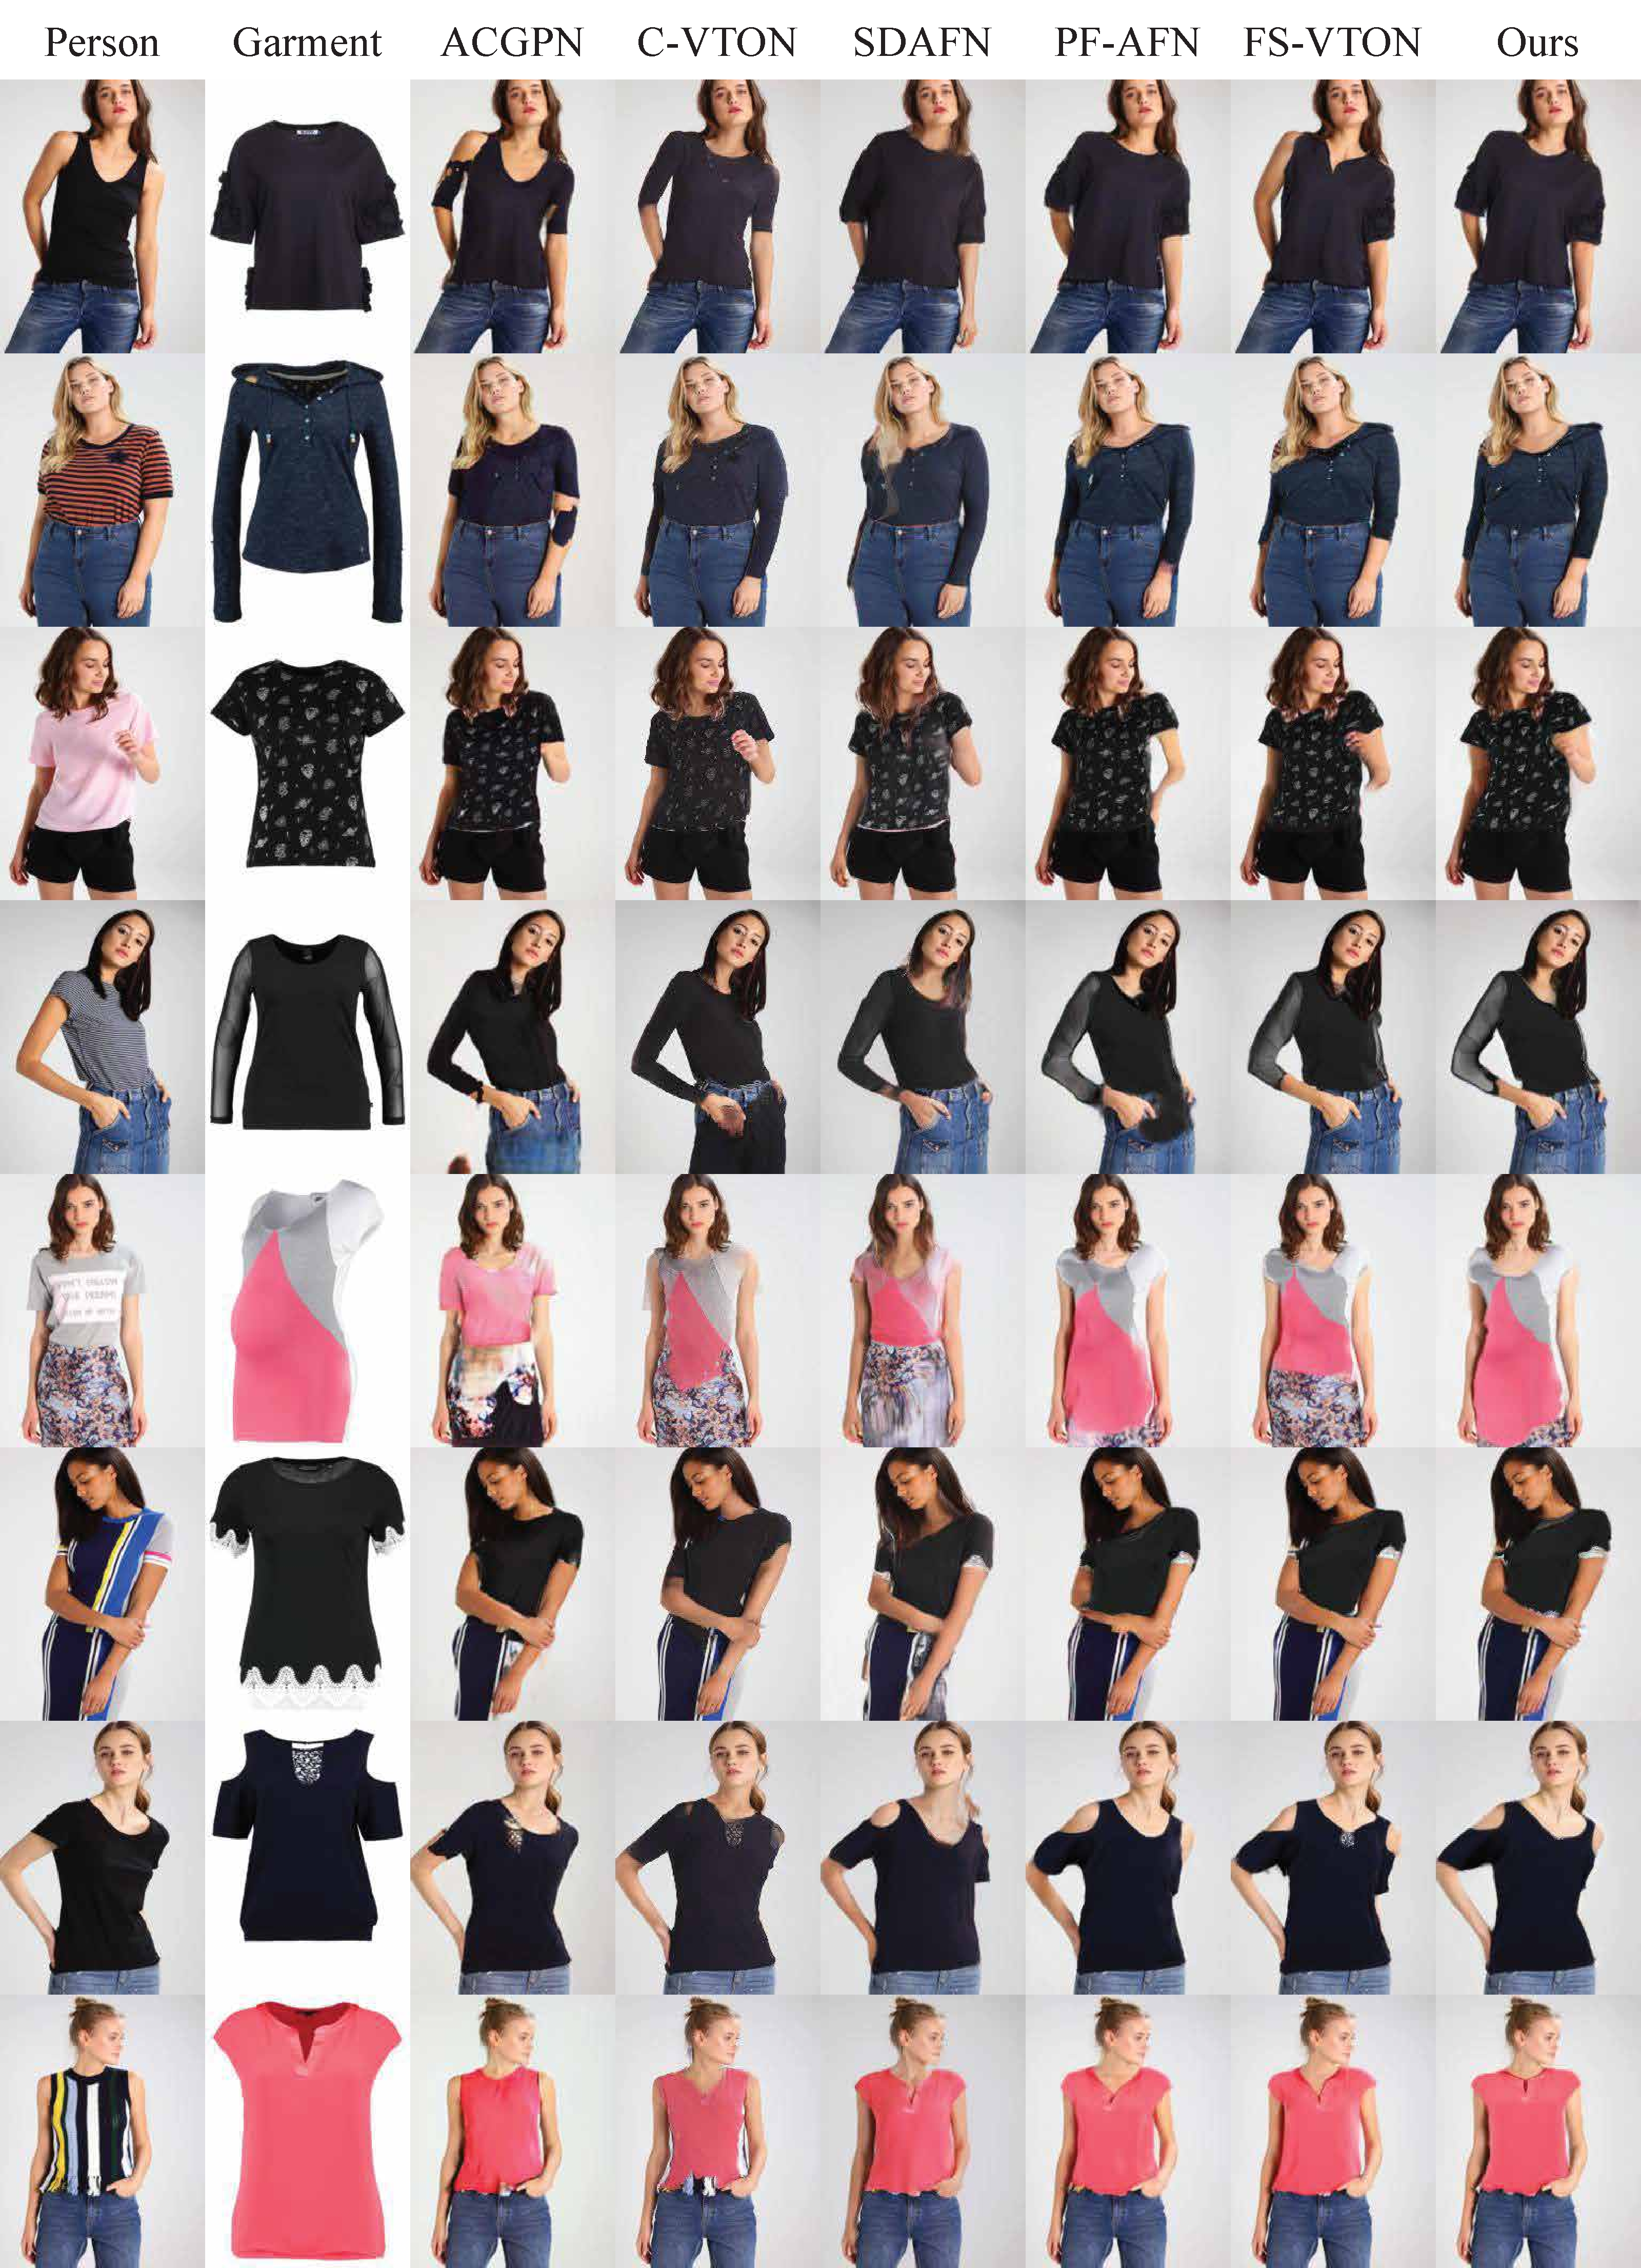
\includegraphics[width=\linewidth]{content/resources/images/tryon/qualitative-viton.pdf}
  \caption{Qualitative comparison on VITON-Clean dataset~\cite{Han-CVPR2018-Viton}.}
  \label{fig:qualitative-viton}
  \vspace{-2mm}
\end{figure}

%%%%%%%%%%%%%%%%%%%%%%%%%%%%%%%%%%%%%%%%%%%%%%%%%%%%%%%%%%%%%%%%
% \section{Fashion Recommendation}
% \subsection{Done}
% \subsubsection{Dataset}
% We conduct our experiments on the PolyvoreOutfits dataset \cite{Mariya-ECCV18-Learning}. The dataset has 251.008 fashion items, with 11 main categories (glasses, shoes, accessories, jewelry, scarves, bottoms, hats, outerwear, tops, bags, and all-body). These main categories are further divided into 153 subcategories with no semantic meaning. The dataset also has 2 subsets: disjoint set and non-disjoint set. The disjoint set has 35.140 outfits, and the non-disjoint set has 68.306 outfits. An item can appear in multiple outfits. The disjoint set has a stricter rule about the appearance of an item, each item can only be seen in one of the train/validation/test sets. Meanwhile, in the non-disjoint set, an item can appear in all train/validation/test sets. To limit the scope, we only use the disjoint set. \autoref{fig:disjoint-categories} shows the number of items in each category in the disjoint set.

% \begin{figure}[h!]
%   \centering
%   \includegraphics[width=0.7\linewidth]{Recommendation/disjoint_category.png}
%   \caption{Histogram of categories in the disjoint set}
%   \label{fig:disjoint-categories}
% \end{figure}

% \subsubsection{Fine-tuning metrics}
% To evaluate the recommendation quality between our finetuned models, we use the metric recall at K with the following setups, for each masked item:
% \begin{enumerate}
%     \item Find K items within the same category as the masked item.
%     \item If those K items contain the masked item, count as correct.
% \end{enumerate}
% The final result is the number of correct items / number of masked items * 100.

% \subsubsection{Loss function} We compare 2 losses: Mean Squared Error (\autoref{fig:mse-loss} and Contrastive loss (\autoref{fig:contrastive-loss}). We train the model by randomly masking 1 item in each outfit of the training set, and we validate the model by randomly masking 1 item in each outfit of the validation set. We find that MSE loss is faster to converge but the recall is relatively low, even at higher recall rank. Meanwhile, the contrastive loss still can converge more and also achieve higher recall.

% \begin{figure}[h!]
%   \centering
%   \includegraphics[width=0.7\linewidth]{Recommendation/MSE loss, mask 1.png}
%   \caption{MSE loss, train set (top), validation set (bottom)}
%   \label{fig:mse-loss}
% \end{figure}

% \begin{figure}[h!]
%   \centering
%   \includegraphics[width=0.7\linewidth]{Recommendation/Contrastive, mask 1.png}
%   \caption{Constrastive loss, train set (top), validation set (bottom)}
%   \label{fig:contrastive-loss}
% \end{figure}

% \subsubsection{Normalization the output} Before searching the query vector in the dataset, we have to normalize it. With the same mask setup as above, when conducting some experiments, we discover that normalizing the vector before calculating the loss harms the model. 
% \autoref{fig:contrastive-loss} shows the result of normalizing before feeding to the loss, \autoref{fig:contrastive-loss-no-norm} is the results of normalization after that. When removing the last normalization during the training process, we can get higher recall and also some signs of overfitting.

% \begin{figure}[h!]
%   \centering
%   \includegraphics[width=0.7\linewidth]{Recommendation/Contrastive, mask 1, no norm.png}
%   \caption{Constrastive loss w/o normalization, train set (top), validation set (bottom)}
%   \label{fig:contrastive-loss-no-norm}
% \end{figure}

% \subsubsection{Mask percentage} As our problem is to predict multiple categories at once, we try increasing the mask percentage. We train our model while masking 50\% of items in each outfit of the training dataset and perform the validation by masking 1 item in each outfit of the validation dataset. The result is shown in \autoref{fig:contrastive-loss-no-norm-mask-half}. The validation recall is still the same as when we only mask 1 item, which means the model can learn even with fewer input items. We further evaluate the best validation model on the test dataset with different mask ratios and recall ranks, as shown in \autoref{fig:test-mask-ratio}. The recall drops significantly when we mask 70\% of the items while slowly drops when masking fewer items.


% \begin{figure}[h!]
%   \centering
%   \includegraphics[width=0.7\linewidth]{Recommendation/Contrastive, mask half, no norm.png}
%   \caption{Constrastive loss w/o normalization, mask 50\%, train set (top), validation set (bottom)}
%   \label{fig:contrastive-loss-no-norm-mask-half}
% \end{figure}

% \begin{figure}[h!]
%   \centering
%   \includegraphics[scale=0.4]{Recommendation/Masked ratio.png}
%   \caption{Test set recall by masked ratio}
%   \label{fig:test-mask-ratio}
% \end{figure}

% \subsubsection{SOTA metric}
% Current State-of-the-art papers \cite{Yen-CVPR2020-Fashion, Han-ECCV2022-FashionViL, Sarkar-CVPRW2022-OutfitTransformer} use a subset of the PolyvoreOutfits test set for evaluation, proposed by \cite{Yen-CVPR2020-Fashion}. They calculate the recall at rank K on the fill-in-the-blank problem:
% \begin{enumerate}
%     \item For each outfit, choose 1 item to mask. (the mask item id is predefined, not randomly)
%     \item Find K items within the same subcategory as the masked item.
%     \item If those K items contain the masked item, count as correct.
% \end{enumerate}
% The final result is the number of correct items / number of masked items * 100. The comparison between our model and other SOTA methods is shown in \autoref{table:outfit-SOTA-compare}. This shows that our model cannot achieve as high results as their methods in the single-item fill-in-the-blank problem. 

% \begin{table}[h!]
% \centering
% \begin{tabular}{l c c c}
% \hline
%                                  & K = 10        & K = 30         & K = 50         \\ \hline
% Type-Aware \cite{Mariya-ECCV18-Learning}           & 3.66          & 8.26           & 11.98          \\
% CSA-Net \cite{Lin2020}              & 5.93          & 12.31          & \textbf{17.85} \\
% FashionVIL \cite{Han-ECCV2022-FashionViL}           & 5.83          & \textbf{12.61} & 17.49          \\
% OutfitTransformer   \cite{Sarkar-CVPRW2022-OutfitTransformer} & \textbf{6.53} & 12.12          & 16.64          \\ 
% Ours                             & 4.19          & 8.55           & 11.96          \\ \hline
% \end{tabular}
% \caption{Recall between our methods and other SOTA}
% \label{table:outfit-SOTA-compare}
% \end{table}

% The histogram of the false negative results is shown in \autoref{fig:neg-sample-category}. It looks like the \autoref{fig:disjoint-categories} a lot, especially the "shoes" and "bags" categories. The higher the number of items in a category, the easier to recommend false negative items. \autoref{fig:neg-sample} shows some false negative samples. From our perspective, the recommendation results are still acceptable. Everyone has different tastes in fashion, so the ground truth items may not be the most compatible items for everyone.

% \begin{figure}[h!]
%   \centering
%   \includegraphics[scale=0.2]{Recommendation/neg_sample_by_categories.png}
%   \caption{False negative histogram by categories}
%   \label{fig:neg-sample-category}
% \end{figure}

% \begin{figure}[h!]
%   \centering
%   \includegraphics[width=0.8\linewidth]{Recommendation/neg-samples.png}
%   \caption{False negative samples, the true positive items are colored red, each following line is the recommendation result}
%   \label{fig:neg-sample}
% \end{figure}

% \subsection{Doing}
% \subsubsection{Replace KNN with ANN} We prepare a dataset include 774400 images (from \cite{Mariya-ECCV18-Learning, Liu-CVPR2016-DeepFashion}, extract their embeddings using \cite{Baldrati-CVPR2022-Effective} pretrained CLIP models. We conduct our experiments with the following settings:
% \begin{enumerate}
%     \item Search space: 30K items, 70K items, 300K items, full dataset (774k items)
%     \item Query item: randomly select one item in the search space.
%     \item Algorithms: KNN\footnote{\label{faiss}https://github.com/facebookresearch/faiss}, LSH\footref{faiss}, IVF\footref{faiss}, IVF+PQ\footref{faiss}, HNSW\footref{faiss}, ANNOY\footnote{https://github.com/spotify/annoy}
%     \item Metrics: Search time, memory usage, recall at rank 100 (KNN results as the ground truth)  
% \end{enumerate}

% \blue{Note}:
% LSH: get saturaion point value
% IVF + Annoy: get until 0.98 recall
% IVFPQ: Use IVF params with maximize number of sub vectors
% HSNW: min to get 0.98 recall

% \subsection{To do}
% \subsubsection{Human studying}
% As our problem, recommending multiple categories at the same time, is novel. There have been no metrics or datasets to evaluate the search quality. Also, everyone has different tastes in their fashion style. We plan to perform human studying on 15 people (more is better) whether they find the complementary items compatible with the query item. The metric is calculated as (the number of compatible items / the number of items asked).